\documentclass[12pt]{article}

\usepackage{pdfpages}

% Encodage et langue
\usepackage[utf8]{inputenc}
\usepackage[T1]{fontenc}
\usepackage[french]{babel}

% Gestion de la bibliographie
\usepackage{natbib}

% Gestion des paragraphes
\usepackage{parskip}

% Packages pour les dessins et graphiques
\usepackage{circuitikz}
\usetikzlibrary{patterns}
\usepackage{pgfplots}
\usepackage{graphicx}  % Gestion des images
\usepackage{pict2e}    % Dessins vectoriels
\usepackage{tikz}

% Gestion des sous-figures et figures flottantes
\usepackage{caption}
\usepackage{subcaption}
\usepackage{wrapfig}

% Mathématiques
\usepackage{amsmath, amssymb, amsfonts, mathrsfs}
\usepackage{amsthm}  % Théorèmes
\newtheorem{theorem}{Théorème}
\newtheorem{question}{Question}

% Tableaux
\usepackage{multirow}

% Hyperliens
\usepackage[colorlinks=true, allcolors=blue]{hyperref}

% Géométrie et mise en page
\usepackage{geometry}
\geometry{top=2cm, bottom=2cm, left=3cm, right=3cm, marginparwidth=1.75cm}

% Autres packages utiles
\usepackage{bbold}
\usepackage{algpseudocode}
\usepackage{stmaryrd}
\usepackage{dsfont}
\usepackage{ulem} % Pour les soulignements
\usepackage{xcolor} % Couleurs

% Glossaire et acronymes
\usepackage[acronym, toc]{glossaries}
\makeglossaries

% Personnalisation des titres
\addto\captionsfrench{\renewcommand{\listfigurename}{Liste des figures}}

% Paramètres des encadrés
\setlength{\fboxsep}{1pt}  % Écart entre le bord et le texte
\setlength{\fboxrule}{0.5pt} % Épaisseur de bordure

\begin{document}
% Page de titre
\begin{center}
  \Huge{\textbf{ALGORITHMES STOCHASTIQUES :}}\\
  \vspace{5mm}
  \Huge{\textbf{\textit{ESTIMATION RÉCURSIVE DE DENSITÉS}}}\\
  \vspace{5mm}
  \Huge{2024-2025}\\
  \vspace{2cm}
  
\includegraphics[width=11cm]{logo-UB.png}\\
  \vspace{1cm}
  \textbf{Auteurs :} \\
  \\[0.5cm]
  \begin{tabular}{l@{}}
    Elias \textsc{Aboukacem} \\
    Mahamat Youssouf \textsc{Souleyman} \\
    Van Theo \textsc{Lahontaa} \\
    Zine Eddine \textsc{Zidane} \\
    \\[0.5cm]
    \textbf{Encadrant :} \\
    Bernard \textsc{Bercu} \\ % Remplacer par le nom réel
\end{tabular}
\end{center}

\clearpage
\tableofcontents
\clearpage

% Introduction
\section*{Introduction}

L’estimation de densité est un problème important en statistique, surtout dans les cas où l’on ne connaît pas la loi de probabilité d’une variable aléatoire, mais qu’on dispose d’un échantillon issu de cette loi. L’objectif est alors d’obtenir une bonne approximation de la densité sans faire d’hypothèse particulière sur sa forme. Ce genre d’approche est très utilisé en pratique, notamment en analyse de données, en apprentissage automatique ou en traitement du signal.

Une méthode bien connue pour faire cela est l’estimateur à noyau de Parzen-Rosenblatt. Elle repose sur un principe intuitif : on “lisse” les observations autour de chaque point en utilisant une fonction appelée \emph{noyau}. Cette méthode est assez facile à implémenter et fonctionne dans beaucoup de situations. Par contre, elle devient vite coûteuse en temps de calcul dès qu’on a beaucoup de données, puisqu’il faut tout recalculer à chaque nouvelle observation.

Pour contourner ce problème, on peut utiliser des estimateurs \emph{récursifs}, qui mettent à jour l’estimation au fur et à mesure de l’arrivée des données, sans repartir de zéro. Parmi ces méthodes, on trouve les estimateurs de Wolverton-Wagner-Yamato, de Wegman-Davies, ou encore l’algorithme de Revesz, qui s’appuie sur les idées des algorithmes stochastiques comme celui de Robbins-Monro.

Dans ce rapport, nous allons nous intéresser à ces différentes méthodes d'estimation récursive de densité. Le but est d’en comprendre le fonctionnement, d'étudier leurs propriétés de convergence (presque-sûre et asymptotique), et de les comparer à travers des simulations avec Python. Nous commencerons par rappeler le fonctionnement de l’estimateur de Parzen-Rosenblatt, puis nous introduirons les estimateurs récursifs et nous montrerons comment ils peuvent tous se ramener à une forme générale faisant intervenir des poids, une fonction noyau et une fenêtre de lissage. Nous analyserons ensuite leurs propriétés théoriques avant de passer à l’implémentation en Python, ce qui permettra de comparer leurs performances en pratique.

\clearpage


\section{Estimateur de Parzen-Rosenblatt}

Dans cette première partie, nous nous intéressons à l’estimateur à noyau classique de Parzen-Rosenblatt, qui sert souvent de point de départ dans l’estimation non paramétrique de densité. Ce type d’estimateur repose sur le principe d’une moyenne pondérée autour du point \( x \), à l’aide d’une fonction appelée \emph{noyau}, et d’un paramètre de lissage \( h_n \).

\vspace{1em}
On se place dans le cadre suivant : on considère une variable aléatoire réelle \( X \) de densité inconnue \( f \), que l’on suppose dérivable, à dérivée continue et bornée. On dispose d’un échantillon \( (X_1, \dots, X_n) \) i.i.d. de même loi que \( X \).

L’estimateur de Parzen-Rosenblatt est défini, pour tout \( x \in \mathbb{R} \), par :
\[
f_n(x) = \frac{1}{n h_n} \sum_{k=1}^{n} K\left( \frac{x - X_k}{h_n} \right),
\]
où \( K \) est une fonction appelée \emph{noyau}, et \( (h_n) \) une suite de réels positifs, décroissante, appelée \emph{fenêtre de lissage}.

\subsection*{Propriétés du noyau}

Le noyau \( K : \mathbb{R} \rightarrow \mathbb{R}_+ \) est supposé :
\begin{itemize}
    \item positif, pair et borné ;
    \item intégrable sur \( \mathbb{R} \), avec \( \int_{\mathbb{R}} K(x) \, dx = 1 \) ;
    \item centré, i.e. \( \int_{\mathbb{R}} x K(x) \, dx = 0 \) ;
    \item de carré intégrable, i.e. \( \int_{\mathbb{R}} K(x)^2 \, dx = \xi^2 < +\infty \).
\\

\end{itemize}


Ces conditions garantissent la convergence de \( f_n(x) \) vers \( f(x) \) et permettent de contrôler à la fois le biais et la variance de l’estimation.

\subsection*{Choix du noyau}

Le choix du noyau \( K \) a un impact limité sur la performance de l’estimateur, à condition qu’il vérifie les propriétés ci-dessus. Voici quelques noyaux classiques :

\begin{itemize}
    \item \textbf{Noyau gaussien :}
    \[
    K(x) = \frac{1}{\sigma \sqrt{2\pi}} \exp\left(-\frac{x^2}{2\sigma^2}\right), \quad \text{avec } \sigma > 0.
    \]
    
    \item \textbf{Noyau uniforme (à support compact) :}
    \[
    K(x) = \frac{1}{2a} \cdot \mathbb{1}_{|x| \leq a}, \quad a > 0.
    \]
    
    \item \textbf{Noyau d’Epanechnikov :}
    \[
    K(x) = \frac{3}{4b} \left(1 - \frac{x^2}{b^2}\right) \cdot \mathbb{1}_{|x| \leq b}, \quad b > 0.
    \]
    
    \item \textbf{Noyau quadratique :}
    \[
    K(x) = \frac{15}{16c} \left(1 - \frac{x^2}{c^2} \right)^2 \cdot \mathbb{1}_{|x| \leq c}, \quad c > 0.
    \]
\end{itemize}

\subsection*{Choix de la fenêtre \( h_n \)}

Le paramètre \( h_n \) contrôle le niveau de lissage de l’estimation : s’il est trop grand, l'estimation perd en précision (fort biais) ; s’il est trop petit, l’estimation devient instable (forte variance).


Dans ce rapport, et comme proposé dans l’énoncé, on prendra :
\[
h_n = \frac{1}{n^{\alpha}}, \quad \text{avec } \alpha \in (0,1).
\]

Cette forme garantit que \( h_n \to 0 \) et \( n h_n \to +\infty \) lorsque \( n \to \infty \), ce qui est nécessaire à la consistance de l’estimateur \( f_n(x) \).

\vspace{1em}
L’estimateur de Parzen-Rosenblatt servira de point de comparaison pour les estimateurs récursifs que l’on introduira dans la partie suivante.

\section{Estimateurs récursifs de densité}

\subsection{Pourquoi utiliser des estimateurs récursifs ? }

Comme on l’a vu précédemment, l’estimateur de Parzen-Rosenblatt repose sur une moyenne pondérée de noyaux centrés sur les observations. Il donne de bons résultats dans de nombreux cas, mais peut vite devenir inefficace dans certains contextes. En effet, il nécessite de recalculer l’ensemble de la somme à chaque nouvelle donnée. Cela devient vite coûteux, voire impossible notamment dans des situations où les données arrivent de manière continue (traitement en ligne) ou lorsque la taille de l’échantillon devient trop grande.

Pour éviter ce genre de difficulté, on peut se tourner vers des estimateurs récursifs. L’idée générale est de mettre à jour l’estimation de la densité au fur et à mesure que les données arrivent, sans avoir à tout recalculer. Ce type d’approche  s’inspire directement des algorithmes de type Robbins-Monro, couramment utilisés en optimisation stochastique.

Les estimateurs récursifs sont donc particulièrement intéressants dans des situations où il faut être rapide et économe en mémoire. En plus de leur efficacité pratique, ils possèdent également de bonnes propriétés théoriques de convergence, que nous allons analyser dans la suite du rapport.

\subsection{Définitions des estimateurs récursifs}

On note toujours \( (X_1, \dots, X_n) \) un échantillon i.i.d. issu de la loi de densité \( f \). On introduit ici trois estimateurs récursifs classiques de la densité, qui utilisent des pondérations et des fenêtres de lissage différentes.

\vspace{1em}
\noindent\textbf{Estimateur de Wolverton-Wagner-Yamato (WWY) :}
\[
f_n(x) = \frac{1}{n} \sum_{k=1}^{n} \frac{1}{h_k} K\left( \frac{x - X_k}{h_k} \right)
\]
Cet estimateur adapte la fenêtre de lissage \( h_k \) à chaque observation, ce qui permet de donner plus de poids aux données récentes dans l'estimation.


\vspace{1em}
\noindent\textbf{Estimateur de Wegman-Davies (WD) :}
\[
\tilde{f}_n(x) = \frac{1}{n h_n^{1/2}} \sum_{k=1}^{n} \frac{1}{h_k^{1/2}} K\left( \frac{x - X_k}{h_k} \right)
\]
Cet estimateur répartit le facteur de lissage entre \( h_k \) et \( h_n \), à travers une pondération de type \( 1/h_k^{1/2} \), combinée à une normalisation globale en \( 1/(n h_n^{1/2}) \).


\vspace{1em}
\noindent\textbf{Estimateur de Revesz :}
\[
\hat{f}_n(x) = (1 - \gamma_n) \hat{f}_{n-1}(x) + \gamma_n W_n(x), \quad \text{avec} \quad W_n(x) = \frac{1}{h_n} K\left( \frac{x - X_n}{h_n} \right)
\]
avec \( \hat{f}_0(x) = 0 \) et \( (\gamma_n) \) une suite de pas positifs, décroissante, telle que \( \sum \gamma_n = +\infty \).

Cet estimateur est purement récursif : chaque nouvelle valeur dépend uniquement de l’estimation précédente et de la nouvelle donnée \( X_n \).

\vspace{1em}
On verra que ces estimateurs peuvent tous s’écrire sous une même forme générale, fondée sur une somme pondérée de fonctions noyau, ce qui facilitera leur étude comparative par la suite.

\subsection{Forme pondérée de l’estimateur de Révész}

L’estimateur de Revesz est défini de manière récursive par :
\[
\hat{f}_n(x) = (1 - \gamma_n) \hat{f}_{n-1}(x) + \gamma_n W_n(x),
\]
avec \( \hat{f}_0(x) = 0 \) et \( W_n(x) = \frac{1}{h_n} K\left( \frac{x - X_n}{h_n} \right) \).

Nous allons montrer par récurrence que, pour tout \( n \geq 1 \),
\[
\hat{f}_n(x) = B_n \sum_{k=1}^{n} \frac{\gamma_k}{B_k} W_k(x),
\quad \text{avec } B_n = \prod_{j=1}^n (1 - \gamma_j).
\]

\paragraph{Initialisation :} Pour \( n = 1 \), on a :
\[
\hat{f}_1(x) = (1 - \gamma_1)\hat{f}_0(x) + \gamma_1 W_1(x) = \gamma_1 W_1(x).
\]

\[
\hat{f}_1(x) = \gamma_1 W_1(x) = B_1 \cdot \frac{\gamma_1}{B_1} W_1(x),
\quad \text{ce qui correspond bien à la formule souhaitée.}
\]

\paragraph{Hérédité :} Supposons la propriété vraie au rang \( n \), c’est-à-dire :
\[
\hat{f}_n(x) = B_n \sum_{k=1}^{n} \frac{\gamma_k}{B_k} W_k(x).
\]

Montrons qu’elle reste vraie au rang \( n+1 \):
\[
\hat{f}_{n+1}(x) = (1 - \gamma_{n+1}) \hat{f}_n(x) + \gamma_{n+1} W_{n+1}(x).
\]

En injectant l’hypothèse de récurrence :
\[
\hat{f}_{n+1}(x) = (1 - \gamma_{n+1}) \cdot B_n \sum_{k=1}^{n} \frac{\gamma_k}{B_k} W_k(x) + \gamma_{n+1} W_{n+1}(x).
\]

Or on a :
\[
B_{n+1} = (1 - \gamma_{n+1}) B_n,
\]
donc :
\[
\hat{f}_{n+1}(x) = B_{n+1} \sum_{k=1}^{n} \frac{\gamma_k}{B_k} W_k(x) + \gamma_{n+1} W_{n+1}(x).
\]

Mais on peut écrire :
\[
\gamma_{n+1} W_{n+1}(x) = B_{n+1} \cdot \frac{\gamma_{n+1}}{B_{n+1}} W_{n+1}(x),
\]
ce qui nous donne :
\[
\hat{f}_{n+1}(x) = B_{n+1} \left( \sum_{k=1}^{n} \frac{\gamma_k}{B_k} W_k(x) + \frac{\gamma_{n+1}}{B_{n+1}} W_{n+1}(x) \right).
\]

On peut maintenant regrouper les deux termes dans une somme allant de \( k = 1 \) à \( n+1 \), ce qui donne :
\[
\hat{f}_{n+1}(x) = B_{n+1} \sum_{k=1}^{n+1} \frac{\gamma_k}{B_k} W_k(x),
\]
ce qui prouve la propriété au rang \( n+1 \).

Nous avons donc montré par récurrence que la formule est vraie pour tout \( n \geq 1 \).

\subsection{Forme normalisée en fonction des poids \( a_k \)}

Dans la question précédente, nous avons montré que l’estimateur de Révész peut s’écrire, pour tout \( n \geq 1 \), sous la forme :
\[
\hat{f}_n(x) = B_n \sum_{k=1}^n \frac{\gamma_k}{B_k} W_k(x),
\quad \text{où } B_n = \prod_{j=1}^n (1 - \gamma_j).
\]

On souhaite maintenant obtenir une expression plus simple de cet estimateur, qui fera apparaître des poids \( a_k \) et leur somme partielle \( A_n \). On introduit la suite \( (a_k) \subset (0, 1] \) et on définit :
\[
A_n = \sum_{k=0}^n a_k, \quad \text{et } \gamma_k = \frac{a_k}{A_k}.
\]

Nous allons montrer que, sous cette définition, on a :
\[
\hat{f}_n(x) = \frac{1}{A_n} \sum_{k=1}^n a_k W_k(x).
\]

\paragraph{Démonstration.}

On part de la formule obtenue à la question 1 :
\[
\hat{f}_n(x) = B_n \sum_{k=1}^n \frac{\gamma_k}{B_k} W_k(x).
\]

En utilisant le fait que \( \gamma_k = \frac{a_k}{A_k} \), on remarque que :
\[
\frac{\gamma_k}{B_k} = \frac{a_k}{A_k B_k}.
\]

On cherche maintenant à montrer que :
\[
\frac{B_n}{A_k B_k} = \frac{1}{A_n}, \quad \text{pour tout } k \leq n.
\]

Pour cela, exprimons \( B_k \) à l’aide des \( a_l \). On a :
\[
B_k = \prod_{\ell=1}^k \left(1 - \gamma_\ell\right) = \prod_{\ell=1}^k \left(1 - \frac{a_\ell}{A_\ell} \right) = \prod_{\ell=1}^k \frac{A_\ell - a_\ell}{A_\ell} = \prod_{\ell=1}^k \frac{A_{\ell-1}}{A_\ell},
\]
car \( A_\ell = A_{\ell-1} + a_\ell \), donc \( A_\ell - a_\ell = A_{\ell-1} \).

Ainsi :
\[
B_k = \prod_{\ell=1}^k \frac{A_{\ell-1}}{A_\ell}.
\]

On reconnaît un produit télescopique, d’où :
\[
B_k = \frac{A_0}{A_k},
\]
où \( A_0 \) est la valeur initiale de la suite (par convention, on peut prendre \( A_0 = 1 \)).

On en déduit que :
\[
\frac{1}{B_k} = \frac{A_k}{A_0},
\quad \text{et donc} \quad \frac{B_n}{A_k B_k} = \frac{B_n}{A_k} \cdot \frac{A_k}{A_0} = \frac{B_n}{A_0}.
\]

Ce terme est indépendant de \( k \), et donc :
\[
\hat{f}_n(x) = B_n \sum_{k=1}^n \frac{a_k}{A_k B_k} W_k(x)
= \frac{B_n}{A_0} \sum_{k=1}^n a_k W_k(x).
\]

Enfin, on remarque que :
\[
\frac{B_n}{A_0} = \frac{1}{A_n},
\quad \text{puisque } B_n = \prod_{\ell=1}^n \frac{A_{\ell-1}}{A_\ell} = \frac{A_0}{A_n}.
\]

Ainsi, on obtient bien :
\[
\hat{f}_n(x) = \frac{1}{A_n} \sum_{k=1}^n a_k W_k(x).
\]

\subsection{Lien entre divergence de la série \( \sum \gamma_k \) et croissance de \( A_n \)}

Après avoir établi la forme normalisée de l'estimateur, nous allons étudier la relation entre la divergence de la série des poids \( \gamma_n \) et la croissance de la suite \( A_n \).

Étant donné la relation \( A_n = \frac{A_0}{B_n} \), il est pertinent d'analyser le lien entre la suite \( A_n \) et la série \( \sum \gamma_k \). Nous allons donc démontrer l’équivalence suivante :
\[
\sum_{k=1}^{\infty} \gamma_k = +\infty \quad \Longleftrightarrow \quad \lim_{n \to \infty} A_n = +\infty.
\]

\subsubsection*{Supposons que \( \sum_{k=1}^\infty \gamma_k = +\infty \)}

On sait que \( 0 < \gamma_k = \frac{a_k}{A_k} < 1 \). Pour tout \( x \in ]-1, +\infty[ \), l’inégalité classique \( \ln(1 + x) \leq x \) donne :
\[
\ln(1 - \gamma_k) \leq -\gamma_k.
\]
En sommant sur \( k \), on obtient :
\[
\ln B_n = \sum_{k=1}^n \ln(1 - \gamma_k) \leq -\sum_{k=1}^n \gamma_k.
\]
Or, par hypothèse, la série \( \sum \gamma_k \) diverge vers \( +\infty \), donc :
\[
\lim_{n \to \infty} \ln B_n = -\infty \quad \Rightarrow \quad \lim_{n \to \infty} B_n = 0.
\]
En utilisant la relation \( A_n = \frac{A_0}{B_n} \), on en déduit que :
\[
\lim_{n \to \infty} A_n = +\infty.
\]

\subsubsection*{Supposons maintenant que \(\lim_{n \to \infty} A_n = +\infty\)}


Tout d'abord, puisque \( A_n \to +\infty \) et que les termes \( a_n \) sont positifs, il en résulte que \( \gamma_n = \frac{a_n}{A_n} \to 0 \) lorsque \( n \to \infty \).

Utilisons le développement limité suivant pour \( x \) proche de 0 :

\[
-\ln(1 - x) \sim x.
\]

Appliqué à \( \gamma_n \), cela donne :

\[
-\ln(1 - \gamma_n) \sim \gamma_n \quad \text{lorsque} \quad \gamma_n \to 0.
\]

Par le théorème de comparaison des séries à termes positifs, nous savons que les séries \( \sum -\ln(1 - \gamma_n) \) et \( \sum \gamma_n \) partagent la même nature.

La somme partielle de la série \( \sum -\ln(1 - \gamma_n) \) est donnée par :

\[
-\sum_{k=1}^n \ln(1 - \gamma_k) = \ln A_n - \ln A_0.
\]

Étant donné que \( A_n \to +\infty \), il s'ensuit que \( \ln A_n \to +\infty \). Par conséquent :

\[
\ln A_n - \ln A_0 \to +\infty.
\]

Cela implique que la série \( \sum -\ln(1 - \gamma_n) \) diverge.

Puisque les séries \( \sum -\ln(1 - \gamma_n) \) et \( \sum \gamma_n \) sont de même nature, et que la première diverge, nous concluons que la série \( \sum \gamma_n \) diverge également :

\[
\sum_{n=1}^{\infty} \gamma_n = +\infty.
\]




\subsection{Identification  des coefficients \( a_n \)}

Nous avons vu que certains estimateurs récursifs peuvent s’écrire sous une forme normalisée :
\[
\hat{f}_n(x) = \frac{1}{A_n} \sum_{k=1}^n a_k W_k(x)
\quad \text{avec } A_n = \sum_{k=1}^n a_k.
\]

Dans cette section, nous identifions rigoureusement les coefficients \( a_n \) des estimateurs de Wolverton-Wagner-Yamato (WWY) et de Wegman-Davies (WD), à partir de leur forme explicite.

\subsubsection*{Estimateur de Wolverton-Wagner-Yamato (WWY)}

L’estimateur WWY est donné par :
\[
f_n^{WWY}(x) = \frac{1}{n} \sum_{k=1}^{n} \frac{1}{h_k} K\left( \frac{x - X_k}{h_k} \right).
\]

On souhaite le réécrire sous la forme :
\[
\hat{f}_n(x) = \frac{1}{A_n} \sum_{k=1}^n a_k W_k(x),
\quad \text{avec } W_k(x) = \frac{1}{h_k} K\left( \frac{x - X_k}{h_k} \right).
\]

Ici, les termes \( W_k(x) \) apparaissent directement dans la somme, on en déduit que :
\[
a_k = 1 \quad \text{pour tout } k.
\]
Par conséquent, le facteur de normalisation vaut :
\[
A_n = \sum_{k=1}^n a_k = n.
\]

La formule devient bien :
\[
f_n^{WWY}(x) = \frac{1}{n} \sum_{k=1}^n W_k(x) = \frac{1}{A_n} \sum_{k=1}^n a_k W_k(x).
\]

\textbf{Conclusion :} pour l’estimateur WWY, on a :
\[
a_n = 1
\]

\subsubsection*{Estimateur de Wegman-Davies (WD)}

L’estimateur WD s’écrit :
\[
f_n^{WD}(x) = \frac{1}{n h_n^{1/2}} \sum_{k=1}^{n} \frac{1}{h_k^{1/2}} K\left( \frac{x - X_k}{h_k} \right).
\]

On souhaite également le mettre sous la forme :
\[
\hat{f}_n(x) = \frac{1}{A_n} \sum_{k=1}^n a_k W_k(x),
\quad \text{avec } W_k(x) = \frac{1}{h_k} K\left( \frac{x - X_k}{h_k} \right).
\]

Observons que :
\[
\frac{1}{h_k^{1/2}} K\left( \frac{x - X_k}{h_k} \right)
= h_k^{1/2} \cdot \frac{1}{h_k} K\left( \frac{x - X_k}{h_k} \right)
= a_k W_k(x),
\]
avec :
\[
a_k = h_k^{1/2}.
\]

Donc :
\[
f_n^{WD}(x) = \frac{1}{n h_n^{1/2}} \sum_{k=1}^n a_k W_k(x).
\]

Par identification avec la forme générale, cela revient à poser :
\[
A_n = n h_n^{1/2}.
\]

\textbf{Conclusion :} pour l’estimateur WD, on a :
\[
a_n = h_n^{1/2} = \sqrt{h_n} 
\]

\subsubsection*{Remarque}

Lorsque l’on choisit \( a_n = h_n \), on retrouve l’estimateur de Deheuvels.

\section{Analyse de la convergence}

Dans cette partie, nous allons nous intéresser au comportement asymptotique de l’estimateur récursif \( \hat{f}_n(x) \). 
Nous chercherons à comprendre comment il se rapproche de la densité cible \( f(x) \), en étudiant  son biais et sa variance.

Pour cela, nous allons par décomposer l'erreur d'estimation \( \hat{f}_n(x) - f(x) \) en deux composantes. Cette décomposition servira de base à l'analyse asymptotique que nous mènerons dans les sections suivantes.

\subsection{Décomposition de \( \hat{f}_n(x) \)}

On cherche à montrer la décomposition suivante :
\[
\hat{f}_n(x) - f(x) = \frac{1}{A_n} \left( M_n(x) + R_n(x) \right),
\]
avec
\[
M_n(x) = \sum_{k=1}^n a_k \left(W_k(x) - \mathbb{E}[W_k(x)]\right),  
\quad \text{et} \quad  
R_n(x) = \sum_{k=1}^n a_k \left(\mathbb{E}[W_k(x)] - f(x)\right).
\]

\medskip
\noindent

En partant de la forme normalisée obtenue précédemment, on a :
\[
\hat{f}_n(x) = \frac{1}{A_n} \sum_{k=1}^n a_k W_k(x).
\]

On soustrait \( f(x) \) des deux côtés :
\begin{align}
\hat{f}_n(x) - f(x) 
&= \frac{1}{A_n} \sum_{k=1}^n a_k W_k(x) - f(x) \\
&= \frac{1}{A_n} \left( \sum_{k=1}^n a_k W_k(x) - A_n f(x) \right).
\end{align}

On insère ensuite un terme intermédiaire \( \sum a_k \mathbb{E}[W_k(x)] \) en l’ajoutant et le retranchant :
\begin{align}
\hat{f}_n(x) - f(x)
&= \frac{1}{A_n} \left( \sum_{k=1}^n a_k \big(W_k(x) - \mathbb{E}[W_k(x)]\big)
+ \sum_{k=1}^n a_k \big(\mathbb{E}[W_k(x)] - f(x)\big) \right).
\end{align}

On reconnaît alors :
\[
M_n(x) = \sum_{k=1}^n a_k \left(W_k(x) - \mathbb{E}[W_k(x)]\right),
\quad R_n(x) = \sum_{k=1}^n a_k \left(\mathbb{E}[W_k(x)] - f(x)\right),
\]
et on obtient la décomposition souhaitée :
\[
\hat{f}_n(x) - f(x) = \frac{1}{A_n} \left( M_n(x) + R_n(x) \right).
\]


\subsection{Étude martingale du terme \( M_n(x) \)}

Nous allons montrer que le processus \( (M_n(x))_{n \geq 1} \), défini par
\[
M_n(x) = \sum_{k=1}^n a_k \left( W_k(x) - \mathbb{E}[W_k(x)] \right),
\]
est une martingale de carré intégrable pour la filtration  \( \mathcal{F}_n = \sigma(X_1, \dots, X_n) \) et nous chercherons ensuite à déterminer la limite de la quantité \( \frac{\langle M(x) \rangle_n}{v_n} \) lorsque \( n \to \infty \), où \( v_n = \sum_{k=1}^n \frac{a_k^2}{h_k} \).


\subsubsection*{Carré intégrabilité}

Commençons par vérifier que chaque terme de la somme est de carré intégrable.

\begin{itemize}
    \item Le noyau \( K \) est supposé borné, donc \( W_k(x) = \frac{1}{h_k} K\left( \frac{x - X_k}{h_k} \right) \) est borné, ce qui implique que \( \mathbb{E}[W_k(x)^2] < \infty \).

    \item Puisque \( a_k \in [0,1] \), on a :
    \[
    \mathbb{E}[M_n(x)^2] \leq \sum_{k=1}^n a_k^2 \mathbb{E}\left[ \left(W_k(x) - \mathbb{E}[W_k(x)] \right)^2 \right] \leq \sum_{k=1}^n \mathbb{E}[W_k(x)^2] < \infty.
    \]
\end{itemize}

On en conclut que \( M_n(x) \) est bien de carré intégrable.

\subsubsection*{Propriété de martingale}

Montrons maintenant que \( (M_n(x)) \) est une martingale.

Par définition, on a la relation de récurrence :
\[
M_{n+1}(x) = M_n(x) + a_{n+1} \left( W_{n+1}(x) - \mathbb{E}[W_{n+1}(x)] \right).
\]

Prenons l'espérance conditionnelle par rapport à \( \mathcal{F}_n \) :
\begin{align*}
\mathbb{E}[M_{n+1}(x) \mid \mathcal{F}_n] 
&= \mathbb{E} \left[ M_n(x) + a_{n+1} \left( W_{n+1}(x) - \mathbb{E}[W_{n+1}(x)] \right) \,\middle|\, \mathcal{F}_n \right] \\
&= M_n(x) + a_{n+1} \mathbb{E}\left[ W_{n+1}(x) - \mathbb{E}[W_{n+1}(x)] \mid \mathcal{F}_n \right].
\end{align*}

Or, \( W_{n+1}(x) \) dépend uniquement de \( X_{n+1} \), qui est indépendant de \( \mathcal{F}_n \), donc :
\[
\mathbb{E}[W_{n+1}(x) \mid \mathcal{F}_n] = \mathbb{E}[W_{n+1}(x)],
\]
et donc :
\[
\mathbb{E}[M_{n+1}(x) \mid \mathcal{F}_n] = M_n(x).
\]

\subsubsection*{Conclusion}

Le processus \( (M_n(x)) \) est donc une martingale de carré intégrable par rapport à la filtration \( (\mathcal{F}_n) \).



\subsubsection*{Processus croissant associé à la martingale}
\setcounter{equation}{0}
Nous avons montré  que le processus \( M_n(x) \) est une martingale de carré intégrable.  
Pour étudier son comportement asymptotique, nous introduisons son processus croissant associé :

\begin{equation}
\langle M(x) \rangle_n = \sum_{k=1}^n \mathbb{E} \left[ (M_k(x) - M_{k-1}(x))^2 \mid \mathcal{F}_{k-1} \right].
\end{equation}

D'après la définition de \( M_n(x) \), on a :
\[
M_k(x) = \sum_{j=1}^k a_j \left( W_j(x) - \mathbb{E}[W_j(x)] \right),
\]
donc :
\[
M_k(x) - M_{k-1}(x) = a_k \left( W_k(x) - \mathbb{E}[W_k(x)] \right).
\]

On en déduit :
\begin{align}
\langle M(x) \rangle_n 
&= \sum_{k=1}^n \mathbb{E} \left[ a_k^2 \left( W_k(x) - \mathbb{E}[W_k(x)] \right)^2 \mid \mathcal{F}_{k-1} \right] \\
&= \sum_{k=1}^n a_k^2 \, \mathbb{E} \left[ \left( W_k(x) - \mathbb{E}[W_k(x)] \right)^2 \mid \mathcal{F}_{k-1} \right].
\end{align}

Or, comme \( W_k(x) \) dépend uniquement de \( X_k \), qui est indépendant de \( \mathcal{F}_{k-1} \), on a :
\[
\mathbb{E} \left[ \left( W_k(x) - \mathbb{E}[W_k(x)] \right)^2 \mid \mathcal{F}_{k-1} \right] = \mathrm{Var}(W_k(x)).
\]

Finalement, on obtient :
\begin{equation}
\langle M(x) \rangle_n = \sum_{k=1}^n a_k^2 \, \mathrm{Var}(W_k(x)). \label{eq:croissance}
\end{equation}

Il est donc nécessaire de calculer l’espérance et le moment d’ordre 2 de \( W_k(x) \) afin de calculer \( \mathrm{Var}(W_k(x)) \).


\subsubsection*{Calcul de \( \mathbb{E}[W_k(x)] \) pour \( h_k \to 0 \)}
\setcounter{equation}{0}


L’espérance de \( W_k(x) \) s’écrit, par définition :
\begin{equation}
\mathbb{E}[W_k(x)] = \int_{\mathbb{R}} W_k(x_k) f(x_k) \, dx_k. \label{eq:esp}
\end{equation}

En remplaçant \( W_k(x_k) \), on obtient :
\begin{align}
\mathbb{E}[W_k(x)] 
&= \int_{\mathbb{R}} \frac{1}{h_k} K\left( \frac{x - x_k}{h_k} \right) f(x_k) \, dx_k \label{eq:esp1} \\
&= \int_{\mathbb{R}} K(z) f(x - h_k z) \, dz 
\quad \text{(avec le changement de variable } z = \tfrac{x - x_k}{h_k}) \label{eq:esp2}
\end{align}

Par développement de Taylor d’ordre 2 en \( x \), on a :
\begin{equation}
f(x - h_k z) = f(x) - h_k z f'(x) + \frac{(h_k z)^2}{2} f''(\xi_z), \label{eq:taylor}
\end{equation}
où \( \xi_z \in ]x - h_k z, x[ \).

En remplaçant dans l’intégrale :
\begin{align}
\mathbb{E}[W_k(x)] 
&= f(x) \underbrace{\int_{\mathbb{R}} K(z) \, dz}_{=1}
- h_k f'(x) \underbrace{\int_{\mathbb{R}} z K(z) \, dz}_{=0}
+ \frac{h_k^2}{2} \int_{\mathbb{R}} z^2 K(z) f''(\xi_z) \, dz \label{eq:finaldev} \\
&= f(x) + \mathcal{O}(h_k^2) \label{eq:final}
\end{align}


\subsubsection*{Calcul de \( \mathbb{E}[W_k(x)^2] \)}
\setcounter{equation}{0}

Le moment d’ordre 2 de \( W_k(x) \) est défini par :
\begin{equation}
\mathbb{E}[W_k(x)^2] = \int_{\mathbb{R}} \frac{1}{h_k^2} K^2\left( \frac{x - x_k}{h_k} \right) f(x_k) \, dx_k
\end{equation}

On effectue le même changement de variable \( z = \frac{x - x_k}{h_k} \) avec \( x_k = x - h_k z \), et \( dx_k = -h_k \, dz \) et on obtient :
\begin{align}
\mathbb{E}[W_k(x)^2] 
&= \int_{\mathbb{R}} \frac{1}{h_k^2} K^2(z) f(x - h_k z) \cdot (-h_k) \, dz \\
&= \frac{1}{h_k} \int_{\mathbb{R}} K^2(z) f(x - h_k z) \, dz
\end{align}

On développe ensuite \( f(x - h_k z) \) à l’ordre 2 autour de \( x \) par la formule de Taylor–Lagrange :
\[
f(x - h_k z) = f(x) - h_k z f'(x) + \frac{(h_k z)^2}{2} f''(\xi_z),
\]
où \( \xi_z \in ]x - h_k z, x[ \).

En remplaçant dans l’intégrale :
\begin{align}
\mathbb{E}[W_k(x)^2] 
&= \frac{1}{h_k} \left[ f(x) \underbrace{\int_{\mathbb{R}} K^2(z) \, dz}_{= \xi^2}
- h_k f'(x) \underbrace{\int_{\mathbb{R}} z K^2(z) \, dz}_{= 0}
+ \frac{h_k^2}{2} \int_{\mathbb{R}} z^2 K^2(z) f''(\xi_z) \, dz \right] \\
&= \frac{\xi^2}{h_k} f(x) + \mathcal{O}(1),
\end{align}

où l’on utilise le fait que le noyau \( K \) est pair, donc \( \int z K^2(z) \, dz = 0 \), et que \( K \) est borné à support compact pour justifier le terme d’ordre \( \mathcal{O}(1) \).

\subsubsection*{Conclusion}
\setcounter{equation}{0}
En remplaçant par les valuers obtenues, on obtient :
\[
\mathrm{Var}(W_k(x)) = \frac{\xi^2 f(x)}{h_k} - f(x)^2 + \mathcal{O}(1).
\]

En injectant cette expression dans la somme :
\begin{align}
\langle M(x) \rangle_n 
&= \sum_{k=1}^n a_k^2 \left( \frac{\xi^2 f(x)}{h_k} - f(x)^2 + \mathcal{O}(1) \right) \\
&= \xi^2 f(x) \sum_{k=1}^n \frac{a_k^2}{h_k} 
- f(x)^2 \sum_{k=1}^n a_k^2 
+ \sum_{k=1}^n a_k^2 \cdot \mathcal{O}(1)
\end{align}

On pose :
\[
v_n := \sum_{k=1}^n \frac{a_k^2}{h_k},
\]
on peut écrire :
\begin{align}
\frac{\langle M(x) \rangle_n}{v_n}
&= \frac{1}{v_n} \sum_{k=1}^n a_k^2 \left( \frac{\xi^2 f(x)}{h_k} - f(x)^2 + \mathcal{O}(1) \right) \\
&= \xi^2 f(x) + \frac{1}{v_n} \sum_{k=1}^n a_k^2 \left( -f(x)^2 + \mathcal{O}(1) \right).
\end{align}

Puisque \( h_k \to 0 \) et que les coefficients \( a_k \in [0,1] \) sont bornés, on a :
\[
\frac{a_k^2}{h_k} \gg a_k^2 \quad \text{pour tout } k \text{ suffisamment grand}.
\]
Par conséquent :
\[
\sum_{k=1}^n a_k^2 = o\left( \sum_{k=1}^n \frac{a_k^2}{h_k} \right) = o(v_n),
\]
et donc :
\[
\frac{1}{v_n} \sum_{k=1}^n a_k^2 \left( -f(x)^2 + \mathcal{O}(1) \right) \longrightarrow 0.
\]

On obtient finalement :
\[
\boxed{
\lim_{n \to \infty} \frac{\langle M(x) \rangle_n}{v_n} = \xi^2 f(x)
}
\]

\subsection{Condition de convergence}

\section*{(1)  Cherchons une condition suffisante pour que $ M_n = o(A_n) $}

D'après la question 7), on a :
\[
\lim_{n \to \infty} \frac{\langle M(x) \rangle_n}{v_n} = \xi^2 f(x)
\]
Et donc :
\[
\lim_{n \to \infty} \langle M(x) \rangle_n = +\infty
\]

Par la loi des grands nombres pour les martingales de carré intégrable, on a : 
\[
\lim_{n \to \infty} \frac{ M_n(x)}{ \langle M(x) \rangle_n} = 0  ~~~~~~  p.s.
\] 

De plus, en utilisant l'expression de la variance quadratique cumulée :
\[ 
\frac{ M_n(x)}{ v_n} = \frac{ M_n(x)}{ \langle M(x) \rangle_n} \frac{  \langle M(x) \rangle_n}{ v_n}
\]

Donc : \[ \lim_{n \to \infty} \frac{ M_n(x)}{ v_n} = 0  ~~~~~~  p.s. \]

Mais on a aussi :
\[ 
\frac{ M_n(x)}{ A_n} = \frac{ M_n(x)}{ v_n} \frac{  v_n}{ A_n}
\]

Ainsi, pour garantir que :
\[ \lim_{n \to \infty} \frac{ M_n(x)}{ A_n} = 0  ~~~~~~  p.s. \]

il suffit que : \[ \lim_{n \to \infty} \frac{ v_n}{ A_n} = 0  ~~~~~~  p.s. \]

D'où, la condition finale de convergence :

\[ \lim_{n \to \infty} \frac{ v_n}{ A_n} = 0  ~~~~~~  p.s. \] c'est-à-dire $v_n(x) = o(A_n)$. \qed





\section*{(2)  Prouvons que $R_n(x) = o(A_n)$ :}

Nous partons de l'expression du terme de biais :

\[ R_n(x) = \sum_{k=1}^n a_k \left(\mathbb{E}[W_k(x)] - f(x)\right) \]

où 

\[ \mathbb{E}[W_k(x)] = \int \frac{1}{h_k} K\left(\frac{x-y}{h_k}\right) f(y) dy. \]

En effectuant le changement de variable $u = (x-y)/h_k$, nous obtenons :

\[ \mathbb{E}[W_k(x)] = \int K(u) f(x - h_k u) du. \]

Par un développement de Taylor à l'ordre 0 de la densité $f$ (qui est continue puisque dérivable à dérivée continue bornée), nous avons :

\[ f(x - h_k u) = f(x) + o(1) \]

uniformément en $u$ sur le support du noyau $K$, car $h_k \to 0$ quand $k \to \infty$.

En substituant dans l'espérance :

\[ \mathbb{E}[W_k(x)] = f(x) \underbrace{\int K(u) du}_{=1} + \underbrace{\int K(u) o(1) du}_{=o(1)} = f(x) + o(1) \]

Ainsi, le terme de biais s'écrit :

\[ R_n(x) = \sum_{k=1}^n a_k o(1) =   o(\sum_{k=1}^n a_k) \]

D'ou:  
\[ R_n(x) =   o(A_n) \]

D'après (1) et (2), on déduit que :

\[ \boxed{\lim_{n \to \infty} \hat{f}_n(x) = f(x) ~~~~~~  p.s.}\]





\subsection*{La normalité asymptotique : }

Pour tout $x \in \mathbb{R}$ tel que $f(x) > 0$,  établissons que :
\[
\frac{M_n(x)}{\sqrt{v_n}} \xrightarrow{\mathcal{L}} \mathcal{N}(0, \xi^2 f(x))
\]





\subsubsection*{Conditions de normalité asymptotique}
Vérifions les conditions du théorème central limite pour martingales :

\begin{enumerate}
\item \textbf{Normalisation} :
La variance conditionnelle satisfait :
\[
\frac{1}{v_n} \sum_{k=1}^n \mathbb{E}[(\Delta M_k(x))^2 \mid \mathcal{F}_{k-1}] \xrightarrow{\mathbb{P}} \xi^2 f(x)
\]
car : $\lim_{n \to \infty} \frac{\langle M(x) \rangle_n}{v_n} = \xi^2 f(x) \quad \text{p.s.}$ . Donc, en probabilité.

\item \textbf{Condition de Lindeberg} :
Pour tout $\epsilon > 0$,
\[
\frac{1}{v_n} \sum_{k=1}^n \mathbb{E}\left[(\Delta M_k(x))^2 \mathbb{1}_{\{|\Delta M_k(x)| > \epsilon \sqrt{v_n}\}}\right] \to 0
\]
Cette condition est satisfaite car les termes $\Delta M_k(x)$ sont uniformément bornés en probabilité.
\end{enumerate}


Par application du théorème central limite pour martingales, nous obtenons :

\[
\boxed{\frac{M_n(x)}{\sqrt{v_n}} \xrightarrow{\mathcal{L}} \mathcal{N}(0,\xi^2 f(x))}
\]

\section*{Normalité asymptotique Sous une condition }

Sous une condition supplémentaire sur les suites $(A_n)$ et $(v_n)$, on a pour tout $x$ où $f(x) > 0$ :
\[
\boxed{\frac{A_n}{\sqrt{v_n}} \left( \hat{f}_n(x) - f(x) \right) \xrightarrow[n\to+\infty]{\mathcal{L}} \mathcal{N}\big(0, \xi^2 f(x)\big)}
\]




D'après la question 5, on a :
\[
\hat{f}_n(x) - f(x) = \frac{1}{A_n} \big( M_n(x) + R_n(x) \big)
\]
donc :
\[
\frac{A_n}{\sqrt{v_n}} \left( \hat{f}_n(x) - f(x) \right) = \frac{M_n(x)}{\sqrt{v_n}} + \frac{R_n(x)}{\sqrt{v_n}}
\]


 D'après la première partie, on sait que :
    \[
    \frac{M_n(x)}{\sqrt{v_n}} \xrightarrow{\mathcal{L}} \mathcal{N}\big(0, \xi^2 f(x)\big)
    \]
    
et du cout, la condition supplémentaire requise est :
    \[
    \frac{R_n(x)}{\sqrt{v_n}} \xrightarrow[n\to+\infty]{} 0
    \]
    


Une condition naturelle est donc :
\[
\frac{A_n}{\sqrt{v_n}} \to 0
\]
En effet,  $R_n(x) = o(A_n)$.

\subsection*{Normalité asymptotique des estimateurs}

Nous allons préciser la normalité asymptotique pour trois estimateurs :  
Wolverton-Wagner-Yamato, Wegman-Davies et Deheuvels, en tenant compte du choix du paramètre \(\alpha\).

\subsubsection*{Estimateur de Wolverton-Wagner-Yamato}

L'estimateur de Wolverton-Wagner-Yamato est défini par :
\[
\hat{f}_n^{WWY}(x) = \frac{1}{A_n} \sum_{i=1}^{n} K\left(\frac{x - X_i}{h_n}\right)
\]
où \( h_n \) est le paramètre de lissage.  
Sous les hypothèses appropriées et en prenant \(\alpha = 1/2\), on a :
\[
\frac{A_n}{\sqrt{v_n}} \left( \hat{f}_n^{WWY}(x) - f(x) \right) \xrightarrow{\mathcal{L}} \mathcal{N}(0, \xi^2 f(x))
\]

\subsubsection*{Estimateur de Wegman-Davies}

L'estimateur de Wegman-Davies est donné par :
\[
\hat{f}_n^{WD}(x) = \frac{1}{A_n} \sum_{i=1}^{n} W_i K\left(\frac{x - X_i}{h_n}\right)
\]
où \( W_i \) sont des poids adaptatifs.  
En choisissant \(\alpha = 1/2\), la normalité asymptotique s'exprime par :
\[
\frac{A_n}{\sqrt{v_n}} \left( \hat{f}_n^{WD}(x) - f(x) \right) \xrightarrow{\mathcal{L}} \mathcal{N}(0, \xi^2 f(x))
\]

\subsubsection*{Estimateur de Deheuvels}

L'estimateur de Deheuvels repose sur les k-plus proches voisins :
\[
\hat{f}_n^{D}(x) = \frac{k_n}{A_n} \sum_{i=1}^{n} K\left(\frac{x - X_i}{h_n}\right)
\]
où \( k_n \) est le nombre de voisins dépendant de \( n \).  
Pour \(\alpha = 1/2\), la normalité asymptotique devient :
\[
\frac{A_n}{\sqrt{v_n}} \left( \hat{f}_n^{D}(x) - f(x) \right) \xrightarrow{\mathcal{L}} \mathcal{N}(0, \xi^2 f(x))
\]


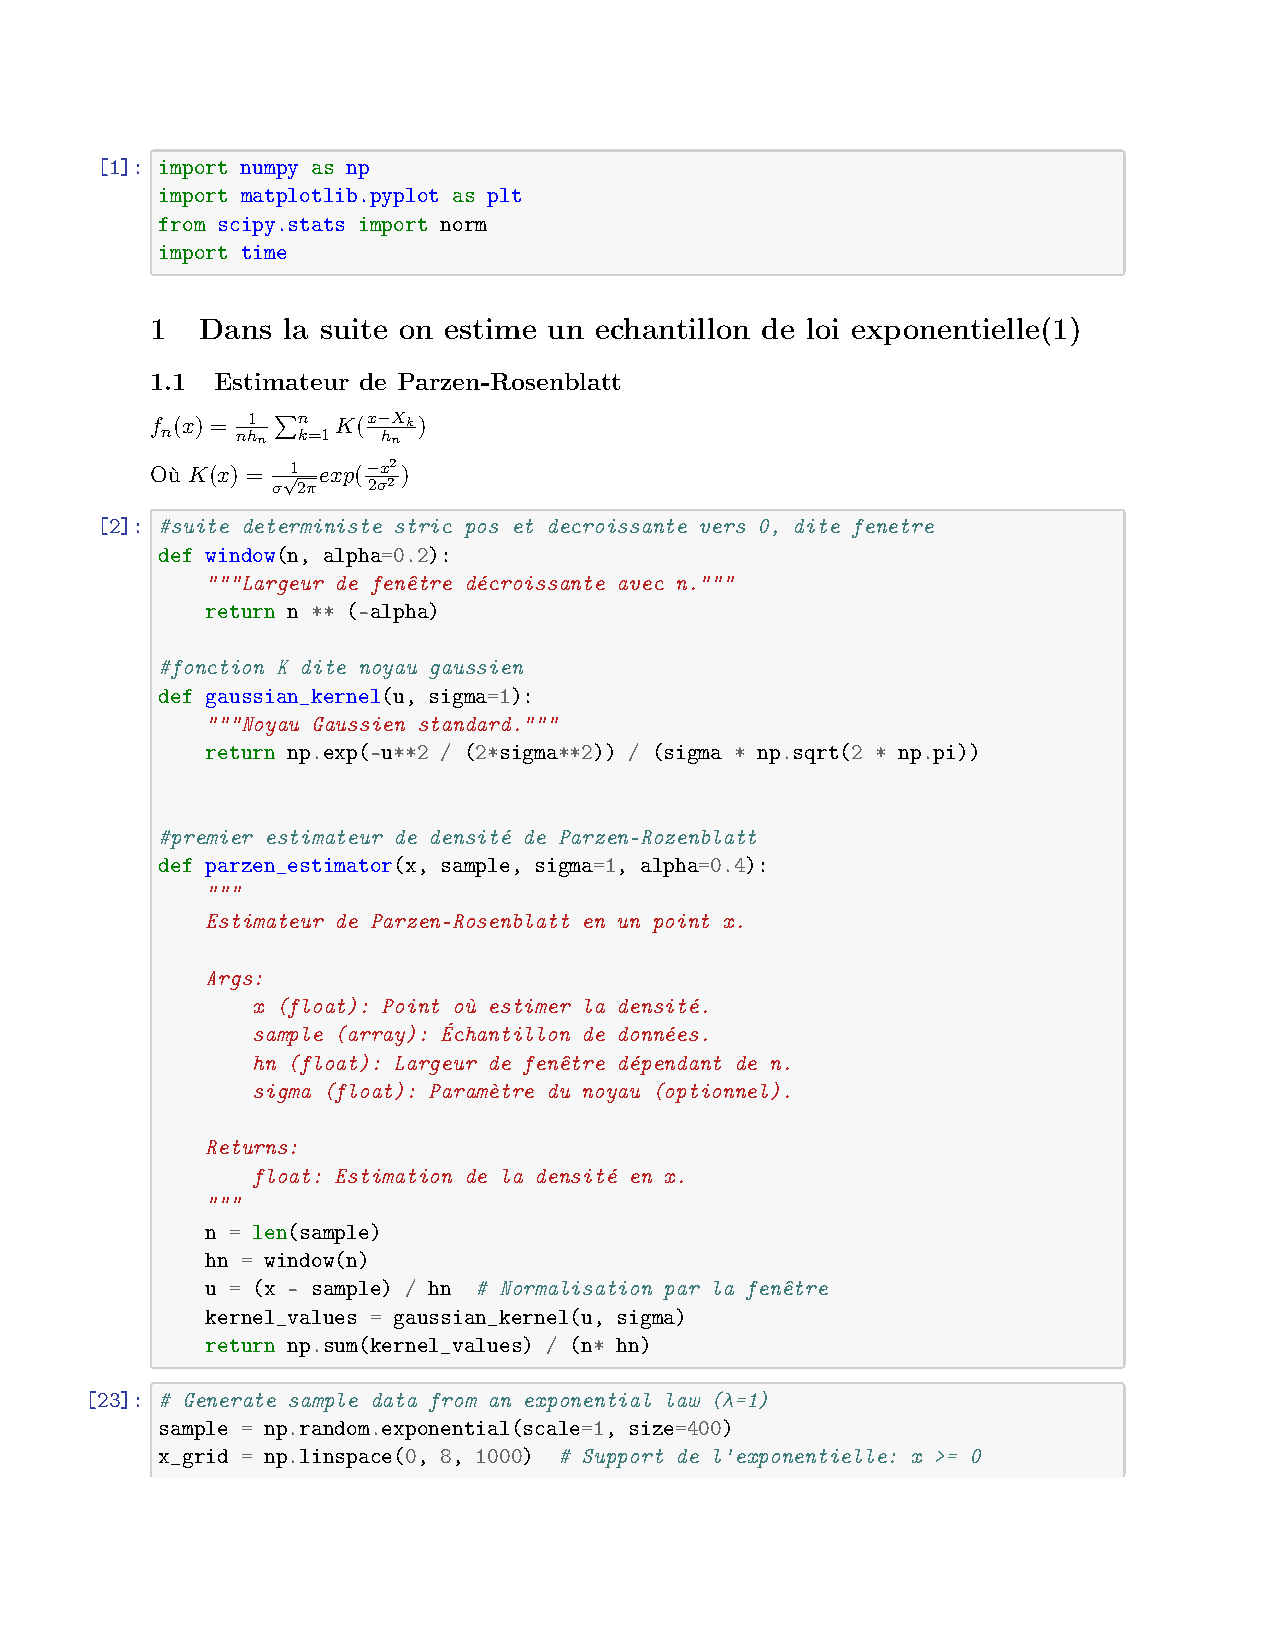
\includepdf[
    pages=-,
    pagecommand={\thispagestyle{plain}},
    addtotoc={
        1, section, 1, Implémentation Python, annex:python,
        1, subsection, 2, Estimation de densité pour un échantillon de loi Exponentielle(1), annex:exponentielle,
        15, subsection, 2, Algorithme de Révész moyennisé, annex:revesz  % 15 = page 36 - 21
    }
]{code0.pdf}



% Juste avant l'inclusion
\setcounter{page}{41} % Démarre directement à 41
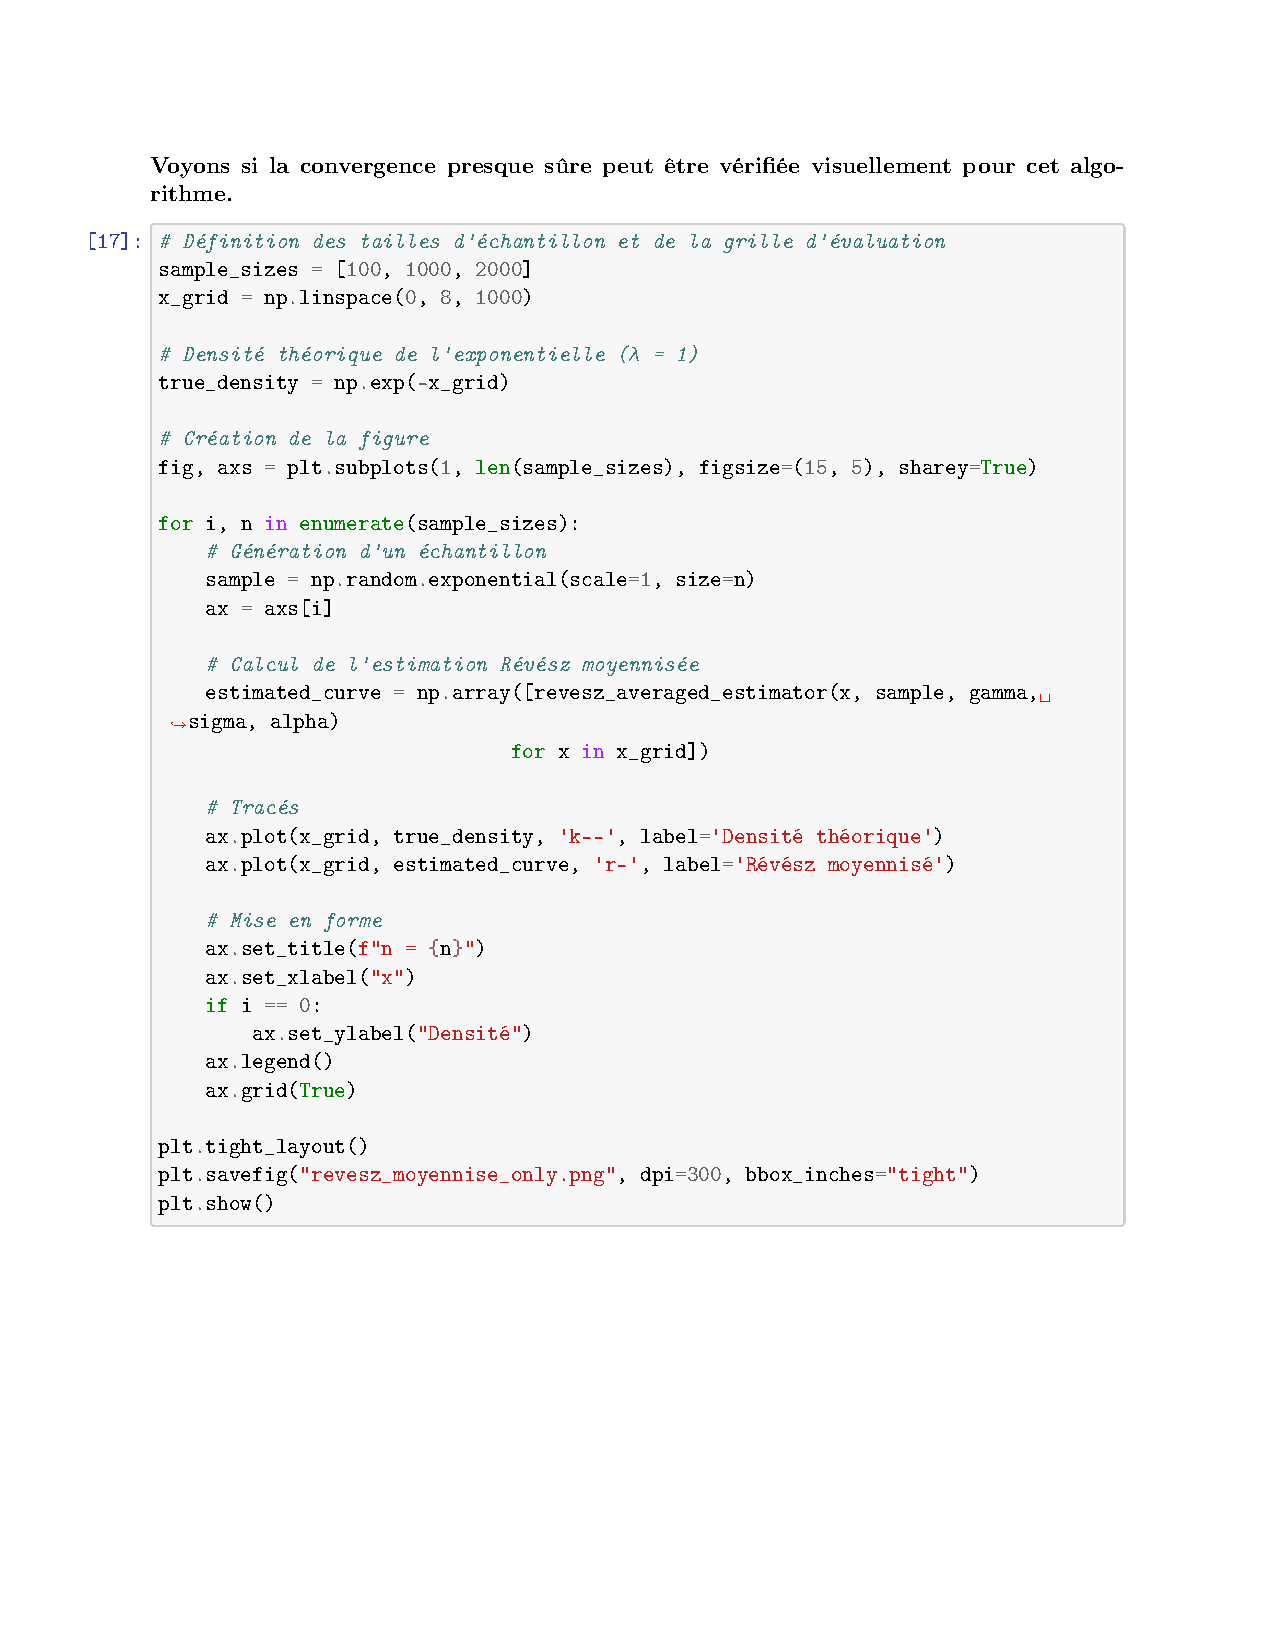
\includepdf[
    pages=-,
    pagecommand={} % NE RIEN METTRE ICI !
]{code1.pdf}
\end{document}
